\chapter{A convincing explanation is not yet an intervention estimate}
\label{closure30:formulation}

A corporate borrower says that a tight credit line prevents it from accepting
an overseas order. A language assistant may recover the relevant passage,
connect it to the financial statements and explain why working capital matters.
The lender still faces a different question: how would a specified change in
credit terms affect exports, repayment and contribution? The answer depends on
why the borrower faces the constraint and what the proposed facility changes.
Good extraction is useful evidence preparation. It does not supply the missing
comparison between alternative lending decisions.

\section{What the financing-and-exports study actually measures}

Li's September 2025 preprint is directly relevant to this distinction. Its
proposed procedure first extracts financing constraints, then export outcomes,
and finally asks a language model to explain a mechanism using economic
theories. The first extraction records a constraint, its severity, supporting
evidence and type. The second records an export metric, value, description and
direction. These explicit intermediate records would help an analyst challenge
an unsupported interpretation of a company report. Equations (1)--(10) define
the information passed between these stages. \citep[Sections 3.1--3.4]{closure30li}

The reported Financing-Export Dataset contains 2,000 Chinese listed firms
over 2015--2019, combining accounts, trade information and text. The stated
comparison uses the same inputs for the proposed prompts and model baselines.
It evaluates financing-constraint classification, subsequent export
participation prediction, repeated-answer consistency and economic relevance
scored by experts. Table~\ref{closure30:exports} reproduces the two rows needed
to understand the claimed improvement; these are the author's reported
scores, not an independently reproduced experiment.

\begin{table}[htbp]
\centering\small
\begin{tabular}{lrrrr}
\toprule
Method & Constraint F1 & Export accuracy & Consistency & Relevance\\
\midrule
Baseline prompts & 0.82 & 76.8\% & 0.78 & 4.1/5\\
Proposed staged prompts & 0.84 & 78.5\% & 0.81 & 4.4/5\\
\bottomrule
\end{tabular}
\caption{Selected reported results from Li's Table 1. The first two columns
measure classification and prediction. Consistency measures repeated outputs;
relevance is an expert assessment of the explanation. None is an estimated
effect of a lending intervention.}
\label{closure30:exports}
\end{table}

The ablation is revealing. Removing the explicit economic-theory guidance
leaves reported F1 and export accuracy at 0.84 and 78.5\%, while consistency
falls to 0.77 and relevance to 3.8/5. This supports the narrower reported
comparison that the guidance changes explanation scores in that experiment.
It does not show that an intervention contrast becomes identified. The
relevance criterion explicitly rewards alignment with economic theory, so
improvement on it is not independent confirmation of the proposed mechanism.
\citep[Sections 4.2.2--4.6; Tables 1--2]{closure30li}

Sections 3 and 4 do not state a treatment-assignment design, a structural
restriction identifying a specified lending effect, or an estimator and
uncertainty interval for that effect. They also do not provide sufficient
model-version, prompt, partition and uncertainty detail to reconstruct the
reported score differences from the paper alone. Those limitations restrict
the use of the evidence; they do not establish that the reported scores are
false. The useful proposal role is a candidate for extracting financial
evidence and developing hypotheses, to be compared on tasks with independently
checked records. Its explanation score cannot value a credit facility.

\section{The same observed story can imply different lending effects}

Consider a deliberately small model in which $F=1$ denotes a financing
constraint and $Y=1$ denotes export participation. Both are binary. For the
moment, suppose every company report states $F$ and $Y$ perfectly, and an
assistant extracts them without error. This assumption gives the assistant
the best possible measurement of these two variables. It lets us isolate the
identification problem from a language model's mistakes.

In the first explanation, an unobserved distress state $U$ causes both the
constraint and the export outcome. Let $U$ be Bernoulli with probability
$1/2$, and let independent errors $E_F,E_Y$ each be Bernoulli with probability
$1/5$. All three inputs are mutually independent. Define
\begin{equation}
 F=U\mathbin{\oplus}E_F,\qquad
 Y=(1-U)\mathbin{\oplus}E_Y,
 \label{closure30:confounded}
\end{equation}
where $\oplus$ is exclusive-or: it flips a binary value when the error is one.
Distress makes the constraint more likely and participation less likely.
Changing $F$ alone leaves the equation for $Y$ unchanged. In this model,
\begin{equation}
 \Pr\{Y=1\mid\doop(F=0)\}
 =\Pr\{Y=1\mid\doop(F=1)\}=\frac12.
 \label{closure30:noeffect}
\end{equation}

The observed contrast nevertheless looks substantial. Symmetry gives
$\Pr(F=1)=1/2$ and $\Pr(U=1\mid F=1)=4/5$. Consequently,
\begin{align}
 \Pr(Y=1\mid F=1)
 &=\frac45\frac15+\frac15\frac45=\frac8{25},\\
 \Pr(Y=1\mid F=0)
 &=\frac45\frac45+\frac15\frac15=\frac{17}{25}.
\end{align}
The participation difference between constrained and unconstrained firms is
$-9/25$, or minus 36 percentage points, even though the intervention effect
is zero. It reflects the unobserved distress composition of the groups.

In the second explanation, financing itself changes participation. Let
$Z$ be Bernoulli with probability $1/2$ and $E$ independently Bernoulli with
probability $8/25$, and set
\begin{equation}
 F=Z,\qquad Y=(1-F)\mathbin{\oplus}E.
 \label{closure30:causal}
\end{equation}
Now the conditional and interventional risks coincide: they are $17/25$
under $F=0$ and $8/25$ under $F=1$. Removing the constraint raises participation
by $9/25$. Both explanations generate exactly the same table of observations:
\begin{center}
\begin{tabular}{crr}
\toprule
 & $Y=0$ & $Y=1$\\
\midrule
$F=0$ & $4/25$ & $17/50$\\
$F=1$ & $17/50$ & $4/25$\\
\bottomrule
\end{tabular}
\end{center}
Each row sums to $1/2$. Exact enumeration of the independent binary inputs
agrees with these algebraic probabilities and with both intervention
calculations. The constants are stipulated for the example; none is an
estimate for Chinese firms or a bank portfolio.

\begin{figure}[htbp]
\centering
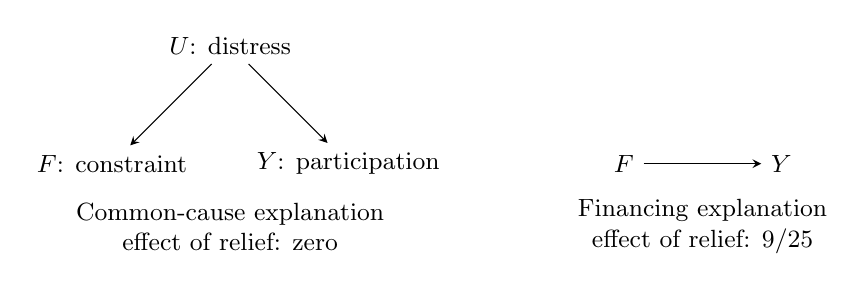
\begin{tikzpicture}[>=stealth,every node/.style={font=\small}]
\node (u) at (0,1.5) {$U$: distress};
\node (f) at (-1.5,0) {$F$: constraint};
\node (y) at (1.5,0) {$Y$: participation};
\draw[->] (u)--(f);\draw[->] (u)--(y);
\node[align=center] at (0,-0.8) {Common-cause explanation\\effect of relief: zero};
\node (f2) at (5,0) {$F$};\node (y2) at (7,0) {$Y$};
\draw[->] (f2)--(y2);
\node[align=center] at (6,-0.8) {Financing explanation\\effect of relief: $9/25$};
\end{tikzpicture}
\caption{The two constructed mechanisms share the observed distribution
of financing constraints and export participation. A report containing only
these facts cannot distinguish their intervention effects.}
\label{closure30:twoworlds}
\end{figure}

Suppose the report is a deterministic transcript $T=t(F,Y)$, recording those
two facts with their values and dates. Then
\begin{equation}
 \Pr(F=f,Y=y,T=t)=\Pr(F=f,Y=y)\,\ind\{t=t(f,y)\}
\end{equation}
is identical in the two explanations. Any fixed extraction or prediction rule
using that information has the same observable performance in both. Random
prompt variation independent of the firm adds no distinction between the two
observational laws. Even an always-consistent explanation can therefore be
attached to two different intervention answers.

Real reports may contain additional information about distress, assignment
or mechanisms. The construction does not exclude that possibility. Such
information must be established and incorporated into the model; a score for
the fluency or plausibility of the resulting explanation cannot substitute
for it. The two effects displayed here demonstrate nonidentification in this
example, not sharp bounds over every compatible causal model.

\section{Knowledge claims need a task-specific test}

Mugleston and colleagues discuss a broader philosophical question: whether
the internal representations of a language model deserve to be called
knowledge. Their argument considers justified true belief, compressed
representations, contextual understanding and the limitations of the Chinese
room analogy. Section 5 also distinguishes informative coherence from merely
repeating an answer, and Section 9 leaves important claims about understanding
unsettled. The paper describes its purpose as a thought experiment.
\citep[Sections 3.3--6 and 9]{closure30mugleston}

That discussion is relevant to how an analyst interprets assistance, but it
does not resolve a lending estimand. A system can organize useful knowledge
without knowing which of the two mechanisms in Figure~\ref{closure30:twoworlds}
generated a particular dataset. Conversely, calling the system a statistical
text generator does not establish that a specific extracted passage is wrong.
The practical assessment concerns the record, the proposed causal restriction
and the decision that follows from it. Philosophical labels cannot replace
those checks.

For a credit decision, the first commitment is an action the lender can carry
out: for example, an offer with specified limit, maturity, price and eligibility
at a fixed date. Setting an abstract constraint indicator to zero is not
automatically that offer. Take-up, competing lenders, borrower responses and
the cost of capital can intervene between the offer and exports. The target
may concern an offered facility, the facility actually drawn, or net
contribution after expected losses. Those quantities require distinct
comparisons.

A useful assisted study would retain the quoted passages and dates, distinguish
the lender's action from the borrower's condition, and set out alternative
causal explanations. An analyst could then defend additional measurements,
a suitable experiment or a credible source of assignment variation. The
evaluation should score faithful extraction, correct formulation and justified
uncertainty separately. A strong extraction score is valuable on its own;
the effect estimate becomes valuable only when its identification and financial
interpretation are also supported.
